%% note: todo's go in todo, as well as optionally in here

\section{Experiment Results}

To test our system, we implemented a prototype client in the Ruby programming language and 
ran experiments using the system, a pool of about 1000 computers scattered world-wide\footnote{It should be noted
that typically only about 300 are active at a time}.
To run each experiment, a central ``driver" program randomly selects members of the pool and instructs them to download a specific url.  To
choose members, the driver first pings known members of PlanetLab to create a list of currently active members.  
It then randomizes this list and uses it in round robin fashion to launch clients
\footnote{If more peers download the file than there are clients available, clients are re-used using the same list in a round-robin fashion, though peer-to-peer connections 
to other peers on the same host are dis-allowed.}. 
Client launch times are generated on after another using a Poisson distribution with an inter-arrival time that is the total startup time
divided by the number of peers.  For example if 1000 peers are expected to enter the system within 100 seconds, it uses a Poisson distribution with 
an average inter-arrival time of 0.1 seconds to start peers, and will finish 
starting them in about 100 seconds\footnote{There is added jitter in start times because some peers have longer latency to establish a TCP connection
to instruct them to start.}  Peers are told the system time when they start a download, 
and use an offset from this start time to log events.  Because of TCP latency in giving them their start times, and system clock skew over time, 
log times can be up to a few seconds off.

Files are downloaded from a well provisioned server at BYU running an Apache2 web server (version 2.2.4) that is
bandwidth limited to 256 KB/s using the mod\_bw module \cite{mod_bw}, and it has a 256 connection limit. 
Experiments run until all peers finish downloading the file. 
Each experiment is repeated 3 times and results are averaged.  A different filename is used for each run, so as to not re-use the same DHT keys.

When peers are done downloading a file, the driver collects their logs and we calculate system statistics.  We measure 
the following:

\begin{enumerate}
\item
Load on the origin server.

This is measured by summing the number of 
bytes received from the origin during each second.  This only measures bytes received from the origin, not necessarily all bytes sent, 
as peers sometimes close their socket connections to the host early, and any data received after the socket has already been closed is dropped by the kernel.  
We disregard the first and last 20\% of entries for this (and other) conglomerate statistics, as the system hasn't reached steady state.
\item
Percent received from the origin.

We also calculate the sum percent of the file received from peers versus from the origin.  This is the number of data bytes that were retrieved
from the origin for any block of the file downloaded, compared to the number of data bytes received from peers during the download.

\item
DHT get, put, and remove times.

We track the time it takes from the start of a DHT operation (initiating TCP contact with a DHT proxy) until an answer is received, for all peers.

\item
Type of peer download.

We also keep track of the way that peers download a given file.  Some peers encounter a fast server and download the entire from the origin.
Some transition to peer-to-peer delivery because of a slow first byte ($T$), and some transition because of a slow origin server speed ($R$).  Some peers 
fail to complete their download (typically those with networks that didn't allow outside connections for some reason).

\end{enumerate}

All box plots show 25th and 75th percentiles, with outlying lines showing 1st and 99th percentiles, and mid-lines showing the median.
For default system parameters, we choose reasonable values of block size of 100 KB, origin minimum speed ($R$) of 128 KB/s, $R$'s calculation window ($W$) 
of 2 seconds, and first-byte timeout ($T$) of 1 second.  Peers download the file from up to 20 other peers at a time ($b$).
Peers linger, serving the file, for 20 seconds after completing a download.

\subsection{Scaling with load}

For our experiments we first test how well our system performs under different loads.
We first run a traditional client-server transfer, to establish a base line from which to compare 
our system. Figure \ref{fig:client_server_download_times} shows the download times for client-server 
downloads, as load increases.  Median download times start at 1.33 seconds with a load of 1 peer/second,
and quickly grow to a high of 344 seconds with a load of 20 peers/second. Download times increase linearly instead 
of exponentially because we start a fixed number of peers and let all downloads complete, without more peers
entering the system.
The top outliers at a load of 20 peers/second typically wait in line around 800 seconds before 
finally receiving the file from the origin. Figure \ref{fig:client_server_server_load} shows that load on the origin server grows quickly to its 
theoretical cap of 250 KB/s under a load of 3 peers/second. Under a load of 20 peers/second, server speed decreases to 203 KB/s, which 
shows the limitations of the rate limiter in that it becomes bursty and less reliable with higher connection rates.

\begin{figure*}
  \begin{center}
    \subfigure[Download times]{
      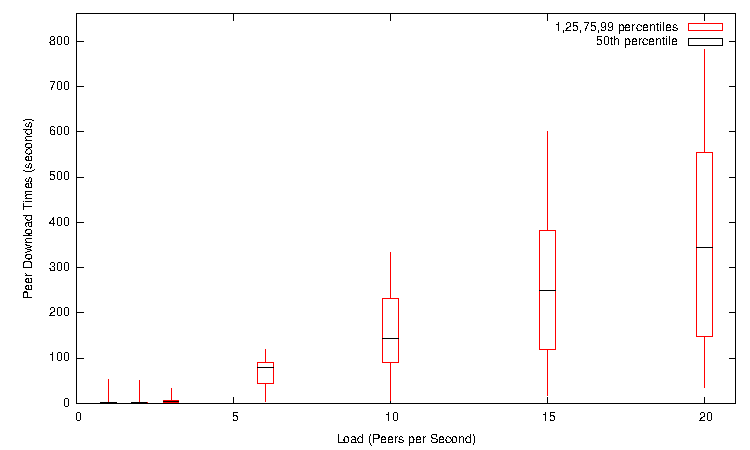
\includegraphics[width=8.5cm]{pics/vr_unnamed316651_cs_stress_test/client_download_Percentile_Line.pdf}
      \label{fig:client_server_download_times}      
    }     
    \subfigure[Load on the origin server]{
      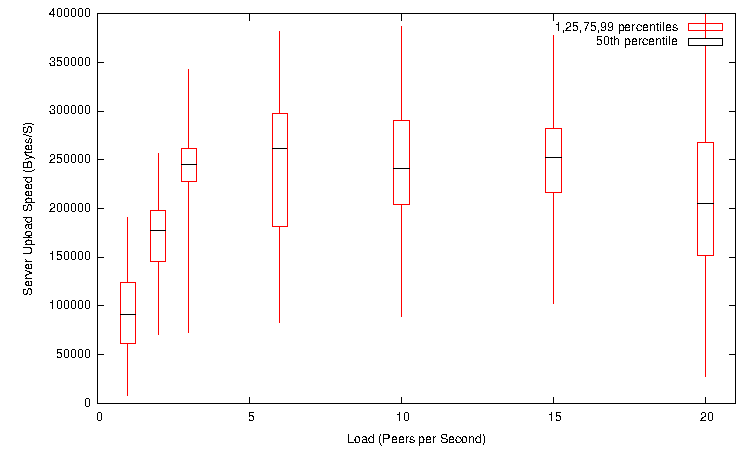
\includegraphics[width=8.5cm]{pics/vr_unnamed316651_cs_stress_test/server_speed_Percentile_Line.pdf}
      \label{fig:client_server_server_load}
    }
    \caption{Traditional client server download under varied load.}  
  \end{center}
\end{figure*}

We next test automatic swarming under the same loads using the default parameters. Figure \ref{fig:yanc} shows that download median times 
start at 1.4 seconds with a load of 1 peer/second, and grow 
to 5.23 seconds with a load of 6 peers/s and 7.46 seconds with 20 peers/s.  Thus download times with swarming are 
30 times faster than for a client-server system.  Download 
The graph's Y axis for download time (Fig. \ref{fig:yanc_download_times}) 
is different than that for client-server (Fig.~\ref{fig:client_server_download_times}) 
because the difference is so great that it would obscure the details. 

We examined our data to determine how clients transition to swarming.  Figure \ref{fig:yanc_death_reasons} shows that at a load of 20 peers/second, 99.5\% 
of peers give up on the origin server because of a slow first byte after one second ($T$). They then query the 
DHT for a peer list, and receive a response with a median latency of 5.2 seconds.  They download the file almost 
immediately once they receive the peer list, hence the median download time of about 7 seconds. 

The amount of peer-to-peer transfer, as expected, increases with higher loads. Under low load clients tend to download 
the file only from the origin.  After a load of about 10 peers/second almost 100\% of the transfer is from 
peers.  At the same time, load drops dramatically on the server (Fig.~\ref{fig:yanc_origin_server_load}).  For lower loads peers start 
downloading the file from the origin, receive some portion of it within the first $W$ (2) seconds, and then
transition to peer-to-peer transfer because the rate of download is less than $R$.  
Thus for the first 2 seconds they are downloading from a slow origin, then they switch to fast peer-to-peer delivery.
The first percentile of download times almost always are the first few clients, who encounter a still fast origin server and download the file directly from it.
Later clients almost always download the file from peers, after encountering a slow origin.

There are two basic causes for why some outlying clients take a long time to download the file.  One is that a few poorly connected clients take so long to download blocks from peers
that their peers finish lingering and drop the existing connections.  These clients then have to request a new 
peer list from the DHT, causing an increase in latency.  This problem is exacerbated by the fact that clients request 
the last block from multiple peers.  This causes 
some redundancy in bytes received, which slows down incoming data, causing slow peers to expire their connections' linger time even more often.
The other factor causing slowdown is a sometimes unresponsive DHT. Typically requests come back quickly, however a few requests will timeout after 60 seconds, 
and peers will end up downloading the entire file from the original server within that 60 seconds, or have to perform a new 
query, and will then download the file normally after that.  We're not entirely sure why this behavior occurs with Bamboo.

<%= figure_directory 'vr_medium_p2p_load_tak4', 'yanc', 'Automatic Swarming under varyied load', {'download_times' => true, 'origin_server_load' => true, 'death_reasons' => true} %>

\subsection{Impact of system parameters}

If a peer can download a file quickly from the origin, it does no help to also download the file from its
peers. Our system accomodates for this by specifying parameters for the conditions under which it will 
transition to a peer-to-peer delivery. We test the impact of varying these and other system parameters, in order 
to explore the dynamics of our system. In each test we start 1000 peers, with an average of 15 peers entering 
the system per second, using a Poisson distribution with an interarrival time of 0.066 seconds (all peers enter the system within 67 seconds). 
Peers download a 100 KB file, using a 100 KB block size, and a connection limit of 5 ($b$), with $R$ set to 128 KB/second and $W$ set to 2 seconds.

We first vary $T$, the timeout for a response byte from the origin server. We expect that an extremely low value 
will cause transitioning too early and an extremely high value 
will cause transitioning too late, both resulting in slow download times. Figure \ref{fig:vary_t_download_times} shows that 
the results hold to our hypothesis. With $T$ set to 0 seconds, median download time is 46.43 seconds. It then drops to 15.35 seconds with $T$ set at 0.75 seconds, 
but rises to 35 seconds with $T$ set to 10 seconds.

Figure \ref{fig:vary_t_death_reasons} shows a break down of the reasons peers transition to peer-to-peer delivery.  $dT$ is the number
of peers who transition to peer-to-peer delivery because of a slow first byte, $dR$ is the number of
peers that transition because of a too low value of $R$, $died$ is the number of peers that never complete the download\footnote{This is 
rare and typically occurs when their host's network has a connectivity problem and it cannot access outside hosts} and $http\_straight$ is the number of peers
that download the entire file from the origin server.

A higher value of $T$ causes $R$ to become more important.  With low values of $T$, almost 100\% of peers transition to peer-to-peer delivery because of $T$. 
With $T$ set to 10 seconds about 80\% of peers transition because of $T$, and 20\% because of $R$, so far fewer.

<%= figure_directory 'vr_unnamed17712_dT', 'vary_t', 'Varying T', {'download_times' => true, 'death_reasons' => true} %>

We next examine the effect of varying $R$, the server's minimum calculated speed.  We vary $R$ from 32 KB/s to 1 MB/s, and set $T$ to a 
reasonably high value of 10 seconds, so that $R$ will be more of a factor in causing peer-to-peer transition. 
The expected result us that too high of values of $R$ will cause peers to transition 
too early, and that values too low will cause peers to transition too late, both resulting in poor performance. Figure \ref{fig:vary_dr} shows that this is the case.
With $R$ at 5 KBps, median download times are 40 seconds, with $R$ at 40 KBps, download times drop to 15 seconds, and reach
a low of 13 seconds with $R$ set to 160 KBps. Higher values than 160 KBps, however, result in slower downloads.  $R$ set to 1 MBps has a median download time of 30 seconds. 

<%= figure_directory 'vr_unnamed502788_dR_fromStart_5000by_fixed_settingAndMajorTimes_8_times_0.0666666666666667s__10s_100000B_255000BPS_5000s_10s_2.0s_100000B', 
  'vary_dr', 'Varying R', 'download_times' => true %> 

We next vary $W$, the amount of recent download time used to calculate $R$. Our hypothesis is that 
a small value for $W$ will cause the calculation to be too sensitive and thus slow download times because it will be inaccurate. 
We vary $W$ from 0.1 seconds 
to 10 seconds and run the same experiment described above, but with $T$ set to 10 seconds and $R$ set to 128 KB/s. Figure \ref{fig:dw} shows the results are 
slightly different than our hypothesis. Varying $W$ does make some difference, but only when set 
to a very low value. Median download times are 17 seconds with $W$ set to 0.25 seconds. For $W$ \textgreater{} 0.25 seconds
median download times stay at approximately 25 seconds. Surprisingly, 
most peers (about 800 out of 1000) still transition to peer-to-peer delivery because of 
a slow first byte ($T$), even with $T$ set to the larger value of 10 seconds. 
The reason for this is that we don't start calculating $R$ until after the first byte is received, and 
in the majority of cases (800/1000) this didn't happen until after $T$ had expired, so $T$ still 
causes most of the transitioning, and appears to be more of a dominant factor overall.  A lower value of $W$ only affects the first 
200 peers, who receive bytes from the non-overloaded origin.  These peers do transition more quickly to peer-to-peer delivery with a lower $W$, but there are few of them.

% ltodo so was it all the first 200 that always transition to R, so that's what sped things up a bit?

% why was this higher, then?

<%= figure_directory '837145_dw', 'dw', 'Varying W', 'download_times' => true %>

\subsection{Effect for a full web page}

We next run an experiment where clients download a full web page.  The normal pattern for a page view 
is to first access some root page which references several other objects, such as images, 
javascript, flash, css, etc. This is the case for a 2007 snapshot of the byu.edu web site, which had a medium sized main page that 
linked to over 10 smaller, objects.  To model this behavior, we run a test where each peer first 
downloads a 100 KB file; when that file completes download each peer then downloads ten other 10 KB files simultaneously 
(from the same origin server), and the total time to download all 11 files is logged. We set the parameters 
to be those mentioned above for testing system parameters, and vary the load from 1 peer/second to 25 peers/second. 

The expected result for this experiment is that downloading multiple pages will be slower than one, 
since it will put more stress on the DHT.  Our results in Figure \ref{fig:multiple_files} prove
this hypothesis correct.  Total download time starts at 1.3 seconds, and grows quickly with higher load, approaching 
150 seconds at a load of 25 peers/second. DHT response times also grow similarly with load.  Median DHT ``put'' times start 
at 0.41 seconds at a load of 1 peer/second, and grow to 12 seconds at a load of 25 peers/second (get and remove times are similar).
This explains some of the download slowdown, because linger time is set to 20 seconds, peer lists are outdated soon after they are created, because
lists take 12 seconds to set, then another 12 seconds to retrieve, and by that time peers may have already gone offline.

% todo is that what really happens though?

<%= figure_directory 'vr_multiples_take_1', 'multiple_files', 'Downloading multiple simultaneous files',  
   {'download_times' => true, 'dht_puts' => true} %>

As Figure \ref{fig:multiple_files_cs_download_times} shows, a client-server system still fares much worse using the same load.  The upper line is the same test using client-server download.

<%= figure 'pics/multiples_p2p_versus_cs_pics/client_download_Percentile_Line.pdf', 
  :caption => 'Comparison of P2P versus client server download times for multiple files', :label => 'fig:multiple_files_cs_download_times' %> 

\subsection{Varying Block Size}

We next measure the effect block size has on download time. We download a 100 KB file with block sizes ranging from 
16 KB to 100 KB, using the same default parameters as specified above for the system tests.
We start 1000 peers at an average of 15 peers entering per second. Figure \ref{fig:vary_block_size} shows that 32 KB blocks result
in the quickest downloads.  This is faster because downloading more blocks allow our system to download 
blocks from several peers simultaneously, without redundancy.  In this case a block size of 32 KB results in a total 3 blocks, and since $b$ by default is 5, all 3 blocks
are downloaded simultaneously. 32 KB blocks were also shown to be most effective in \cite{32_kb_blocks}.

<%= figure_directory 'vr_unnamed240998_blockSize', 'vary_block_size', 'Varying block size', 'download_times' => true  %>

\subsection{Varying linger time}

We next vary the amount of time peers linger, our hypothesis being that a longer linger 
time will speed downloads.  Figure \ref{fig:vary_linger_time} shows our hypothesis is correct.   
We download a 100 KB file, varying linger time from 0 to 160 seconds.
With a linger time of 0 seconds, median download time peaks at 300 seconds, with 
a linger time of 1 second, median download time drops to 127 seconds.  With a linger of 2 seconds, download time further drops to 60 seconds, and
with a linger time of 4 seconds, download time drops to 34 seconds.  Download time stays at about that same level for linger times greater than 4 seconds.

<%= figure_directory 'vr_unnamed497104_linger_fromStart_0by_fixed_settingAndMajorTimes_8_times_0.0666666666666667s__0s_100000B_255000BPS_125000s_1.0s_2.0s_100000B', 
 'vary_linger_time', 'Varying linger time', 'download_times' => true  %> 

\subsection{Downloading Large Files}

We next test our system's ability to download large files. We download a 30 MB file using our system and then again using BitTorrent.
For both systems, block size is set to 256 KB, origin servers are rate limited to 256 KB/second, and linger time 
is set to 0 seconds (though peers share the file while they are still downloading it). 100 peers enter the system at an average of 1 per second.  

The expected result is that the two fare similarly.  Our results, in Table \ref{fig:yanc_vs_bt}, show that a few peers download 
faster with our system, but most download faster with BitTorrent. 
Ours has a slower median time than BitTorrent (847 to 148 seconds), though it has a faster 99th
percentile (982 to 2786 seconds). We're not entirely sure why BitTorrent is faster.  
%One factor affecting our performance is that 
%each peer contacts the origin server in our system.   This can causes full blocks to propagate more slowly into the system.  
% or is the the DHT? why were we slow?
One factor affecting performance is that BitTorrent's seed limits outgoing connections to 7, whereas Apache's connection limit is 256.
This may allow BitTorrent to propagate full blocks more quickly to peers.  BitTorrent's seed also favors peers with higher download 
speeds, which might help propagate blocks,  It uses a dedicated tracker, 
which makes peer rendezvous quicker than using a DHT.  BitTorrent peers use a ``rarest block first" selection policy, enabling them to choose blocks more efficiently.  
These differences may allow it to respond to a flash crowd such as this one better.  In future work our system can be optimized to handle flash crowds such as this better.

One interesting statistic is that the relative download times within each system are similar.
The difference between the 25th and 75th percentile download time in our system is 150 seconds, 
or 5\% of the 75th percentile's time. The difference between the 25th and 75th percentiles in BitTorrent 
is 24 seconds, or 7\% of the 75th percentile's time (a similar percentage). These numbers implies that once 
a few peers have downloaded a file in its entirely, it doesn't take relatively long for the rest of the peers to complete 
the download.  Figure \ref{fig:yanc_30mb_cdf} shows that most of the delivery comes from peers.

<%= figure 'pics/yanc_30mb/yanc_30_mb_cdf.pdf', :caption => 'CDF of percent of file received from peers, 30MB file', :label => 'fig:yanc_30mb_cdf' %>
\small{
\small{
\begin{table}
  \caption{Download times of a 30MB file}
\begin{center}
\begin{tabular}{ c c l }
  Percentiles & Our System (S) & BitTorrent (S) \\
  \hline
  1 & 613 & 131 \\
  25 & 730 & 139 \\
  50 & 847 & 148 \\
  75 & 882 & 163 \\
  99 & 982 & 2786 \\
  \label{fig:yanc_vs_bt}
\end{tabular}
\end{center}
\end{table}
}
}
\subsection{Varying peer connection limit} 

We next vary the maximum number of simultaneous download connections each peer is allowed ($b$). We 
repeat the above 30 MB download experiment, but vary the peer limit from 1 to 50. 
We expect that download times will suffer when the connection limit is too low. Figure \ref{fig:vary_connection_count} shows that, as expected, median 
download times suffer with a low limit, a limit of 1 yielding a median download time of 1604 seconds.  A limit of 16 has a median download time of 931 seconds.  Limits greater than 16 yield
slight improvements.  A 50 peer limit results in a median download time of 875 seconds.

<%= figure_directory 'vr_vary_blocks_large_file', 'vary_connection_count', 'Varying number of concurrent peers' %>
